\documentclass[10pt,a4paper]{article}
\usepackage[a4paper]{geometry}

\usepackage{polski}
\usepackage{xltxtra}
\usepackage{relsize}
\usepackage{fancyvrb}
\usepackage{hyperref}
\hypersetup{
    pdftitle={Sprawozdanie końcowe z projektu indywidualnego z AiSD 2011/2012},%
    pdfauthor={Tomasz Cudziło},%
    colorlinks=true,        % false: boxed links; true: colored links
    linkcolor=black,        % color of internal links
    citecolor=green,        % color of links to bibliography
    filecolor=magenta,      % color of file links
    urlcolor=cyan,          % color of external links
    unicode=true,           % non-Latin characters in Acrobat’s bookmarks
    pdfstartview={FitH},    % fits the width of the page to the window
    pdfnewwindow=true       % links in new window
}
\usepackage{graphicx}
\usepackage{changepage}

%% tweak fonts
\defaultfontfeatures{Mapping=tex-text}
\setromanfont{Charis SIL}
\setsansfont[Scale=MatchLowercase]{Helvetica Neue}
\setmonofont[Scale=MatchLowercase]{Monaco}
\linespread{1.25}

%% define custom commands and environments
\DefineVerbatimEnvironment%
  {SmallVerbatim}%
  {Verbatim}{fontsize=\relsize{-0.5},numbers=left,numbersep=-10pt,frame=lines,tabsize=4}

\newcommand{\f}[1]{\texttt{#1}}
\newcommand{\s}[1]{\textsf{#1}}

\newcommand{\rev}{754330aa66a33e7434e6bda5c083aa3e12b7b65f}
\newcommand{\revhref}[1] {\href{https://github.com/student-tomasz/aisd-projekt-indywidualny/blob/\rev/#1}{\f{#1}}}



\begin{document}

\title{
  Sprawozdanie końcowe z projektu indywidualnego\\
  z przedmiotu Algorytmy i Struktury Danych
}
\author{
  Tomasz Cudziło\\
  \textsc{PW EE Informatyka}\\[7pt]
}
\date{\today}
\maketitle



\section{Opis projektu}

Celem projektu było zaimplementowanie struktury danych przechowującej informacje
o siatce trójwymiarowej i oferującej wydajny dostęp do podstawowych informacji o
jej elementach.

\subsection{Wersja projektu}

Sprawozdanie opisuje projekt w stanie z rewizji \f{\rev}. Opisywany kod źródłowy
jest dostępny do przejrzenia na
\href{https://github.com/student-tomasz/aisd-projekt-indywidualny/tree/\rev}{stronie repozytorium}.



\section{Funkcjonalność}


\subsection{Obsługa}

Program uruchamiany jest komendą:
\begin{SmallVerbatim}
    ruby application.rb sciezka/do/siatki.txt
\end{SmallVerbatim}

Przy pomyślnym wczytaniu pliku z siatką, pojawia się lista dostępnych akcji i
program oczekuje na reakcję użytkownika. Po podaniu identyfikatora akcji i
identyfikatora odpowiedniego elementu, program wyświetla wynik zapytania i
czas jego generacji, oraz zaczyna oczekiwanie na kolejny wybór akcji.

Do wyboru dostępne są wszystkie zapytania wymienione w wymaganiach oraz jedno
dodatkowe: \vspace{10pt}

\begin{SmallVerbatim}
    Akcje: 
     1. indeksy wezlow podanego elementu,
     2. indeksy wezlow bezposrednio sasiadujacych z podanym wezlem,
     3. indeksy elementow bezposrednio sasiadujacych z podanym wezlem,
     4. indeksy krawedzi podanego wezla,
     5. indeksy wezlow podanej krawedzi,
     6. indeksy elementow przyleglych do podanej krawedzi,
     7. indeksy wezlow bezposrednio sasiadujacych z podana krawedzia,
     8. indeksy elementow bezposrednio sasiadujacych z podana krawedzia,
     9. indeksy krawedzi bezposrednio sasiadujacych z podana krawedzia,
     -
     h. pomoc,
     q. koniec. 
\end{SmallVerbatim}


\subsection{Plik wejściowy}

Program wczytuje pliki sformatowane w sposób opisany w wymaganiach projektu.
Metoda parsująca zakłada, że plik jest sformatowany poprawnie i nie przewiduje
obsługi błędów. Struktura pliku, ani spójność wczytanych danych, nie są
walidowane.



\section{Implementacja}


\subsection{Struktura danych siatki}
\label{sub:struktura_danych_siatki}

\subsubsection{Struktura \emph{Half-Edge}}

Podczas planowania projektu i na początku implementacji, zakładałem, że siatka
będzie zaimplementowana jako struktura znana pod nazwą \emph{Half-Edge Mesh}
\cite{half_edge}. Generowanie krawędzi w tej strukturze wymaga przechodzenia
przez wierzchołki trójkątów, zawsze w tym samym kierunku (przy absolutnym
punkcie odniesienia).

Ponieważ w pliku nie były podane wektory normalne trójkątów, naiwnie
żałożyłem, że wybierając kierunek w pierwszym rozpatrywanym trójkącie
``zarażę'' nim pozostałe trójkąty. Moje założenie jest prawdziwe i sprawdza
się dla siatki z pliku \f{meshes/micro.txt}, w której lista trójkątów jest
uszeregowana tak, by każdy następny trójkąt posiadał co najmniej jednego,
rozpatrzonego już sąsiada.

Ten warunek nie jest jednak spełniony dla pozostałych siatek, gdzie można
znaleźć w listach trójkątów przypadki, które nie sąsiadują z trójkątami
znajdującymi się na liście przed nimi.

Przez pewien czas starałem się obejść ten problem (stąd opóźnienie,
przepraszam). Próbowałem wyliczać wektory normalne dla trójkątów, przy
arbitralnie dobranym punkcie i kierunku odniesienia, jednak problem mnie
pokonał i stwierdziłem, że zaimplementuję siatkę jako \emph{Face-Vertex Mesh}
z dodatkową listą krawędzi, opisaną w następnym paragrafie.

W pełni działający kod, z siatką zaimplementowaną na strukturze
\emph{Half-Edge~Mesh} jest dostępny w rewizji
\href{https://github.com/student-tomasz/aisd-projekt-indywidualny/tree/794c2908657a891f020920f34f9f9bc6f5fdb39c}{\f{794c290}}.

\subsubsection{Struktura \emph{Face-Vertex} z krawędziami}

Aktualnie siatka jest zaimplementowana jako standardowa \emph{Face-Vertex
Mesh} z dodatkowymi informacjami o krawędziach wychodzących z każdego
wierzchołka.

Relacje między poszczególnymi składowymi siatki są przedstawione na schemacie
\ref{fig:face_vertex_model} na stronie \pageref{fig:face_vertex_model}.

\begin{figure}[p]
  \centering
  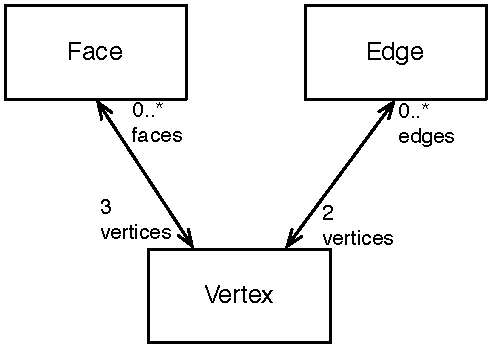
\includegraphics[width=8cm]{figury/face-vertex-model}
  \caption{Schemat zależności pomiędzy składowymi siatki.}
  \label{fig:face_vertex_model}
\end{figure}


\subsection{Struktury pomocnicze}
\label{sec:struktury_pomocnicze}

\subsubsection{Macierz \f{LIL}}
\label{sec:macierz_lil}

W pliku \revhref{lib/matrix/lil.rb} zaimplementowana jest macierz
\f{List-in-List}. Macierze \f{LIL} charakteryzują się dużą oszczędnością
pamięci przy przechowywaniu macierzy rzadkich, oraz wygodnym i wydajnym
wprowadzaniem zmian.

Podczas generowania krawędzi, tworzona jest tymczasowa macierz sąsiedztwa,
która jest zaimplementowana na macierzy \f{LIL}. Dokładny opis zastosowania
znajduje się w paragrafie \ref{sec:generowanie_krawedzi}.

Bezpośrednia implementacja macierzy \f{LIL} w \f{Ruby} polega na
przechowywaniu w tablicy pojedyńczych tablic asocjacyjnych. W przełożeniu na
macierz, wiersze są tablicami asocjacyjnymi, których kluczami są indeksy
kolumn.

Operując na macierzy rzadkiej, efektywny czas dostępu do dowolnej komórki jest
stały. Dostęp do wiersza jest w czasie $O(1)$, ponieważ wiersze są
przechowywane w standardowej tablicy. Dostęp do komórki w wierszu następuje
poprzez tablicę asocjacyjną o efektywnym dostępie $O(1)$, zwłaszcza, że w
pojedynczym wierszu będzie przechowywanych stosunkowo niewiele elementów.

Przyjrzałem się zachowaniu macierzy dla siatki testowej z pliku
\revhref{meshes/large.txt} o~ok.~70 tys. zadeklarowanych trójkątów. Średnia
liczba wartości niezerowych w macierzy sąsiedztwa, wynosiła 10 elementów na
wiersz.

\subsubsection{Tablica haszująca}
\label{sec:tablica_haszujaca}

W plikach z katalogu \revhref{lib/counter\_hash} znajdują się definicje klas
implementujących prostą tablicę haszującą, służącą do zliczania elementów.
Tablica haszująca jest wykorzystywana do znajdowania duplikatów lub przecięć
zbiorów. Szczegółowy opis wykorzystania znajduje się w paragrafie
\ref{sec:wymagane_zapytania}.

Klasa \f{CounterHash::Counter} z pliku \revhref{lib/counter\_hash/counter.rb}
przechowuje referencje do rozpatrywanego obiektu oraz aktualną liczbę wystąpień
tego obiektu.

Instancje klasy \f{CounterHash::Counter} są przechowywane w listach, które są
instancjami klasy \f{CounterHash::Bucket} z pliku
\revhref{lib/counter/bucket.rb}. Są to niesortowane listy jednokierunkowe
zaimplementowane na tablicach. Wyszukiwanie elementu w liście jest $O(n)$,
gdzie $n$ to liczba elementów w liście. Dodawanie elementu również odbywa się
w czasie $O(n)$, ponieważ przed dodaniem nowego elementu, sprawdzane jest czy
element nie znajduje się już w liście.

Dla tablicy haszującej, wydaje mi się, udało osiągnąć się złożoność czasową
wyszukiwania równą $O(1)$. Pozwoliło na to, dobranie odpowiedniej funkcji
haszującej oraz długości tablicy haszującej. Oczywiście w przypadku
pesymistycznym, złożoność czasowa wyszukiwania jest równa $O(n)$. Jest to
przypadek gdy wszystkie elementy tablicy haszującej znajdują się w jednym
koszyku.

Tablica haszująca jest zaimplementowana jako tablica zawierająca referencje do
szestnastu koszyków. Funkcja haszująca wykorzystuje pole \f{id} wyszukiwanego
elementu i zwraca wynik operacji bitowej \f{AND}:

\begin{SmallVerbatim}
    def hash(element)
      return element.id & (buckets.length-1);
    end
\end{SmallVerbatim}

Ponieważ długość tablicy \f{buckets} jest równa $16 == 2^4$, funkcja haszująca
zachowuje się jak maska bitowa dla czterech najmłodszych bitów wartości
\f{id}. W efekcie dla dowolnego argumentu, dostajemy jednoznaczny wynik, w
jednej wydajnej operacji.

Funkcja haszująca zachowuje się dobrze przy danych, które są podawane do
tablicy haszującej w dziedzinie projektu. Tablica jest wykorzystywana przy
znajdowaniu lub usuwaniu duplikatów, z małych (średnio mniej niż
20-elementowych) zbiorów elementów. Elementy rozróżniamy po wartości ich pola
\f{id}. Dodatkowo wiemy, że wartości \f{id} będą występować w grupach o
zbliżonych wartościach (np. rozpatrując zbiory sąsiadów wierzchołków jednej
krawędzi). Dlatego biorąc pod uwagę wyłącznie młode bity z wartości \f{id},
zabezpieczamy się przed nadmierną liczbą kolizji.

Liczba przechowywanych koszyków została wybrana na podstawie średniej liczby
elementów zbiorów, które są wstawiane do do tablicy haszującej.


\subsection{Parsowanie pliku wejściowego}

Parsowanie pliku jest zdefiniowane w metodzie \f{parse\_file} klasy
\f{Mesh::Model} w pliku \revhref{lib/mesh/model.rb}.

Plik jest wczytywany linia po linii. Jako pierwsze, wyszukiwane są dwie linie
spełniające wzorzec na liczbę wierzchołków lub trójkątów. Dopóki obydwie
wartości nie zostaną znalezione, wczytywane linie pliku będą ignorowane. Po
znalezieniu liczb elementów, program przechodzi do pierwszej napotkanej linii
zaczynającej się znakiem \f{\#}. Następnie, program wczytuje ustaloną
wcześniej liczbę linii, umieszczonych bezpośrednio pod aktualną pozycją
kursora pliku.

Linie wczytywane po pierwszej napotkanej linii rozpoczynającej się znakiem
\f{\#}, są interpretowane jako dane wierzchołków, po drugiej jako dane
trójkątów. Bezpośrednio, w trakcie interpretowania poszczególnych linii,
tworzone są obiekty klas odpowiadające danym elementom. Obiekty te są
wstawiane na końce odpowiednich tablic. Wstawianie do tablic odbywa się w
czasie stałym.


\subsection{Przechowywanie składowych siatki}

Klasy stanowiące strukturę siatki są zdefiniowane w plikach z katalogu
\revhref{lib/mesh}. Wierzchołki, trójkąty oraz krawędzie siatki są
reprezentowane odpowiednio przez klasy \f{Mesh::Vertex}, \f{Mesh::Face} oraz
\f{Mesh::Edge}. Wszystkie są agregowane przez klasę siatki \f{Mesh::Model} w
zmodyfikowanych tablicach tj.: \f{Mesh::VerticesHash}, \f{Mesh::FacesHash}
oraz \f{:EdgesHash}.

Klasy \f{Mesh::VerticesHash}, \f{Mash::FacesHash} oraz \f{Mash::FacesHash}
miały z założenia być tablicami haszującymi. Ponieważ po wczytaniu model
siatki nie ulega zmianom, zastosowanie tablicy haszującej nie daje żadnych
zysków w stosunku do zwyczajnej tablicy indeksowanej polami \f{id}
przechowywanych elementów. W efekcje klasy te dziedziczą po standardowej
klasie \f{Array}. Metody dostępu zostały nadpisane, tak by elementy były
przechowywane zaczynając od indeksu 0, nie 1. Dodatkowo dodane zostały metody
pomocnicze \f{add} wstawiające nowoutworzone obiekty składowych siatki na
koniec tablicy.


\subsection{Generowanie połączeń w siatce}

\subsubsection{Generowanie listy trójkątów wierzchołka}

Podczas wykonywania konstruktora klasy \f{Mesh::Face}, następuje iteracja po
wierzchołkach definiujących trójkąt. Każdemu wierzchołkowi trójkąta zostaje
dopisana referencja do aktualnie tworzonego trójkąta. W rezultacie, po
wygenerowaniu całej siatki, każdy wierzchołek posiada listę trójkątów, które
współtworzy.

Zdecydowałem się generować te listy, ponieważ pozwalają na zwrócenie wyniku na
jedno z wymaganych zapytań w czasie stałym. Jednocześnie zdecydowanie
przyspieszają generowanie odpowiedzi na dwa zapytania dotyczące trójkątów
ograniczających i sąsiadujących z daną krawędzią. Szczegóły szukania rozwiązań
na te zapytania są omówione w paragrafie \ref{sec:wymagane_zapytania}.

\subsubsection{Generowanie krawędzi}
\label{sec:generowanie_krawedzi}

Metoda \f{generate\_edges} wywoływana w konstruktorze klasy \f{Mesh::Model}
generuje krawędzie siatki. Dla każdego trójkąta siatki, pobierane są jego
wierzchołki pogrupowane w pary. Dla każdej pary zlecane jest wygenerowanie
krawędzi korzystając z metody \f{Mesh::EdgesHash\#add}.

\begin{SmallVerbatim}
    def generate_edges
      @faces.each do |face|
        face.vertices_ordered.each do |pair|
          @edges.add pair
        end
      end
      @edges.freeze
    end
\end{SmallVerbatim}

Krawędzie są przechowywane w zwykłej tablicy, każda nowa krawędź jest dodawana
na koniec tablicy w czasie stałym. W przeciwieństwie do tworzenia wierzchołków
lub trójkątów, należy sprawdzić, czy krawędź dla aktualnej pary wierzchołków
nie została już stworzona. Służy do tego macierz sąsiedztwa przetrzymywana na
czas generowania krawędzi. Macierz sąsiedztwa jest dla wygody użytkowania
opakowana w klasie \f{Mesh::EdgesJournal}.

Instancja tej klasy jest przechowywana przez \f{Mesh::EdgesHash}, nazwijmy ją
pamiętnikiem. Podczas każdego wywołania metody \f{Mesh::EdgesHash\#add}, w
pamiętniku wyszukiwana jest krawędź identyfikowana parą łączonych przez nią
wierzchołków. Jeśli krawędź została znaleziona, metoda kończy działanie. W
przeciwnym przypadku tworzony jest instancja nowej krawędzi. Referencja do
niej jest zapisywana w tablicy wszystkich krawędzi siatki, a krawedź oznaczana
jako utworzona w macierzy sąsiedztwa.

Dodatkowo klasa \f{Mesh::EdgesJournal} zapewnia efektywne pamięciowo
wykorzystanie macierzy \f{LIL}. Przed każdym odwołaniem się do komórki z
macierzy \f{LIL}, indeksy otrzymanych wierzchołków są sortowane. Dzięki temu
macierz sąsiedztwa jest zapisywana jako macierz trójkątna górna. Bez
sortowania, macierz byłaby symetryczna i potrzebowała dwukrotnie więcej
pamięci.

By powiązać składowe siatki z krawędziami, każdy wierzchołek posiada listę
krawędzi, do których należy. Referencja krawędzi jest dodawana na koniec listy
\f{edges} wierzchołka, w konstruktorze klasy krawędzi. Lista krawędzi
wierzchołka jest analogiczna do listy trójkątów wierzchołka. Rozwiązanie to
może wydawać się mało wydajne pamięciowo.

Początkowo, po zakończeniu generowania miałem zamiar zmieniać wewnątrzną
implementację macierzy sąsiedztwa z macierzy \f{LIL} na macierz \f{CRS}.
Macierz \f{CRS} byłaby wydajnym rozwiązaniem, ponieważ nie byłoby już potrzeby
wprowadzania zmian i jednocześnie odczyt pojedyńczych wierszy wymagałby
jedynie przejścia przez krótki odcinek tablicy. Przetrzymywanie tych
pojedyńczych wierszy, bezpośrednio w odpowiadających im wierzchołkach, wiąże
się z identycznymi kosztami pamięciowymi, natomiast odczyt odbywa się w czasie
stałym, a całe rozwiązanie jest bardziej zorientowane obiektowo. Odczyt całego
wiersza byłby jedyną operacją wykonywaną na macierzy sąsiedztwa, ponieważ jest
równoważny znalezieniu wszystkich krawędzi danego wierzchołka.


\subsection{Wymagane zapytania}
\label{sec:wymagane_zapytania}

Zapytania o numerach 1, 3, 4, 5 to jest: znajdowanie wierzchołków podanego
trójkąta, trójkątów podanego wierzchołka oraz wierzchołków podanej krawędzi i
krawędzi podanego wierzchołka są przechowywane bezpośrednio w strukturze
siatki i są dostępne w czasie stałym. Pozostałe zapytania wymagają
przeprowadzenia operacji o różnym stopniu złożoności.

\subsubsection{Znajdowanie sąsiadów wierzchołka}

Znajdowanie sąsiadów wierzchołka posiada złożoność czasową $O(n)$, gdzie $n$
jest liczbą krawędzi wychodzących z podanego wierzchołka. Sąsiedzi wierzchołka
są znajdowani poprzez przejście przez listę krawędzi wierzchołka i
zapamiętanie drugich końców każdej krawędzi.

\subsubsection{Trójkąty przyległe do podanej krawędzi}

Znajdowanie trójkątów przeległych do krawędzi ma złożoność czasową liniową,
zależną od wielkości sumy trójkątów przyległych do obu końców krawędzi.

Szukany wynik jest przecięciem zbiorów trójkątów przyległych do końców
krawędzi. Do znalezienia przecięcia, wykorzystywana jest tablica haszująca
opisana w paragrafie \ref{sec:tablica_haszujaca}. Najpierw dodawane są do
tablicy haszującej wszystkie trójkąty sąsiadujące z pierwszym z wierzchołków
krawędzi. Następnie iterując po trójkątach drugiego wierzchołka, sprawdzamy
czy aktualny trójkąt znajduje się już w tablicy haszującej. Jeśli tak, jest to
jeden z trójkątów przyległych do danej krawędzi.

W pesymistycznym przypadku całe zapytanie ma złożoność czasową $O(n^2)$,
jednak jest to bardzo rzadki przypadek, gdy identyfikatory wszystkich
przeglądanych trójkątów mają identyczne, cztery najmłodsze bity.

\subsubsection{Wierzchołki i trójkąty sąsiadujące z krawędzią}

Zarówno zbiór wierzchołków i zbiór trójkątów sąsiadujących z krawędzią
wyszukuje się identycznie, opiszę tylko wyszukiwanie trójkątów.

Szukany wynik jest sumą zbiorów trójkątów przyległych do każdego z końców
krawędzi z usuniętymi elementami powtarzającymi się. Znajdujemy ten zbiór,
wstawiając wszytkie rozpatrywane trójkąty do tablicy haszującej. Ponieważ raz
wstawiony trójkąt, nie będzie dodany ponownie, wszystkie elementy tablicy
haszującej są naszym szukanym zbiorem.

Złożność i przypadek pesymistyczny identyczne jak w poprzednim przypadku.

\subsubsection{Krawędzie sąsiadujące z krawędzią}

Znalezienie krawędzi polega na zsumowaniu zbiorów krawędzi wychodzących z
obydwu końców podanej krawędzi i usunięcie z sumy podanej krawędzi.

Zapytanie zaimplementowane jest bez użycia tablicy haszującej, i polega na
wpisaniu do tablicy wyjściowej każdej, oprócz aktualnej, krawędzi.

Złożoność czasowa jest zawsze liniowa, zależna od liczby krawędzi wychodzących
z obu końców danej krawędzi.



\section{Testy}


\subsection{Testy poprawności}

Testy co do poprawności działania struktury siatki przeprowadzane były ręcznie
na siatce z pliku \revhref{meshes/micro.txt}. W pliku opisany jest prosty
sześcian z dodatkowymi punktami pośrodku górnej i dolnej podstawy.


\subsection{Testy wydajnościowe}

Testy wydajnościowe były przeprowadzane z wykorzystaniem biblioteki
\f{perftools.rb} \cite{perftools}. Skrypt profilujący odpowiednie aspekty
alogrytmu znajduje się w pliku \revhref{profiling.rb}. Graficzne interpretacje
profilowania są załączone razem ze sprawozdaniem.

Na grafach aktywności widoczne jest, że wydajność programu w zdecydowanej
części jest ograniczona przez pracę \f{GC}. Reszta aplikacji przeważnie jest
skupiona na operacjach standardowych typów języka \f{Ruby}, do których nie mam
bezpośredniego dostępu.

\subsubsection{Generowanie siatki}

Dokładnie przetestowałem generowanie siatki opisanej w pliku
\revhref{meshes/large.txt}. Jest to siatka składająca się z ok. 70 tysiący
trójkątów.

Średni czas generowania siatki na procesorze \f{2.26GHz Intel Core 2 Duo}
wynosi 2711 ms. W wynikach profilowania możemy zauważyć, że 73.5\% czasu
procesora jest spędzone na obsłudze \f{GC}. Spora część (ok.~15.5\%) jest
spędzona na operacjach przeprowadzanych przez typy wbudowane w standard
\f{Ruby}, do których nie mam dostępu. Są to operacje zapisu do tablic --
metody \f{Array\#[]=} i \f{Array\#<<} łącznie zajmują 4.8\%, lub samo
wczytywanie pliku -- metoda \f{IO\#each} zajmująca 7.6\% czasu procesora.
Pozostały czas --- ok.~11\% jest spędzony na wykonywaniu logiki opisanych
wcześniej struktur.



\begin{thebibliography}{9}
  \bibitem{half_edge}
    \url{http://www.flipcode.com/archives/The_Half-Edge_Data_Structure.shtml}
  \bibitem{perftools}
    \url{https://github.com/tmm1/perftools.rb}
\end{thebibliography}



\end{document}
